% ==============
% COJAC analysis
% ==============

\chapter{COJAC}

\gls{COJAC} \cite{COJAC} est un programme Java permettant de modifier les capacités arithmétiques d'une application Java cible sans en modifier le code. Elle utilise l'API d'instrumentation et peut transformer les classes et méthodes au runtime pour changer le type de calcul effectué. Ainsi, pour changer le type de calculs effectué (ex: nombre réel $\rightarrow$ \gls{Complex-number}), il faut seulement changer l'argument donné à \gls{COJAC} lors du démarrage de l'application. Ceci ne demande aucune modification dans l'application cible.

Ce chapitre détaille tout d'abord les \glspl{Java-agent}, car ils sont essentiels au fonctionnement de \gls{COJAC}. Ensuite, le \gls{Bytecode} Java sera expliqué parce que c'est là-dessus que fonctionne \gls{COJAC}. Finalement, la dernière section explique comment les fonctionnalités supplémentaires désirées peuvent être ajoutés dans \gls{COJAC}.

\section{Agent Java}
\label{sec:agent_java}

Un \gls{Java-agent} est un programme Java spécial conçu pour modifier le comportement d'un autre programme sans en modifier le coude source. C'est sur ce principe fondamental que repose \gls{COJAC}. Comme montré dans la Figure \ref{fig:cojac_classloading}, l'\gls{Java-agent} Java intercepte les fichiers .class qui contiennent du \gls{Bytecode} et peut y apporter des modifications. Le \gls{Bytecode} correspond à l'assembleur de Java. Ce concept est détaillé dans la section \ref{sec:bytecode} suivante.

\begin{minipage}{\linewidth}
    \centering
    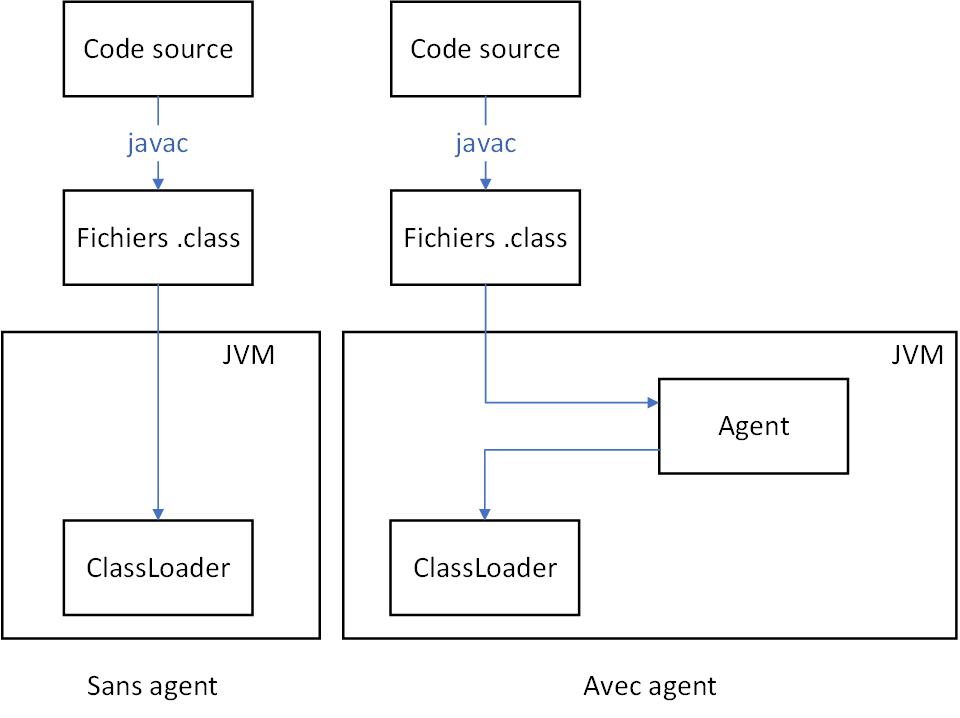
\includegraphics[width=.7\linewidth]{cojac/principle.png}
    \captionof{figure}{Chargement d'une classe}
    \label{fig:cojac_classloading}
\end{minipage}

Cette fonctionnalité est particulièrement utile pour des programmes pouvant fonctionner avec beaucoup d'autres applications. Ils peuvent offrir, par exemple, du monitoring, du profilage, etc.

La majorité des informations dans cette section provient d'une conférence de Rafael Winterhalter \cite{youtube-guide-java-agent}. La première moitié de la conférence se focalise sur la base des \glspl{Java-agent} et des problèmes qui y sont liés. Alors que la seconde moitié se focalise sur Byte Buddy \cite{byte-buddy}, une librairie pour simplifier la transformation de classes.

Il existe deux types d'agents qui seront appelés, dans ce document, agent statique et agent dynamique.

\subsection{Agent statique}

Un agent statique est un \gls{Java-agent} qui est spécifié au démarrage du programme comme c'est le cas avec \gls{COJAC}. Ainsi, lors du démarrage de l'application, l'agent et la \gls{JVM} interagissent ensemble conformément à la Figure \ref{fig:cojac_static_agent}. Cette interaction se déroule en plusieurs étapes:

\begin{enumerate}
    \item La \gls{JVM} appelle l'\gls{Java-agent} en lui donnant le paramètre spécifié (un string) lors du démarrage de l'application. La méthode appelée s'appelle \textit{premain} parce qu'elle est exécutée avant le \textit{main} de l'application cible.
    \item Dans cette méthode \textit{premain}, l'agent doit créer un \textit{ClassFileTransformer}. Cet objet sera utilisé plus tard pour modifié les classes. Cet objet est ensuite donné à la \gls{JVM} grâce à la méthode \textit{Instrumentation.addTransformer}.
    \item Ensuite à chaque fois que la \gls{JVM} veut charger une nouvelle classe, le \textit{ClassLoader} lira le fichier \textit{.class} correspondant.
    \item Le \textit{ClassLoader} enverra ensuite le tableau d'octets qu'il vient de lire au \textit{ClassFileTransformer} qui pourra y apporter les modifications désirées.
    \item Une fois que le \textit{ClassFileTransformer} a modifié la classe, il la retournera la classe à la \gls{JVM}.
\end{enumerate}

\begin{minipage}{\linewidth}% to keep image and caption on one page
\makebox[\linewidth]{%        to center the image
    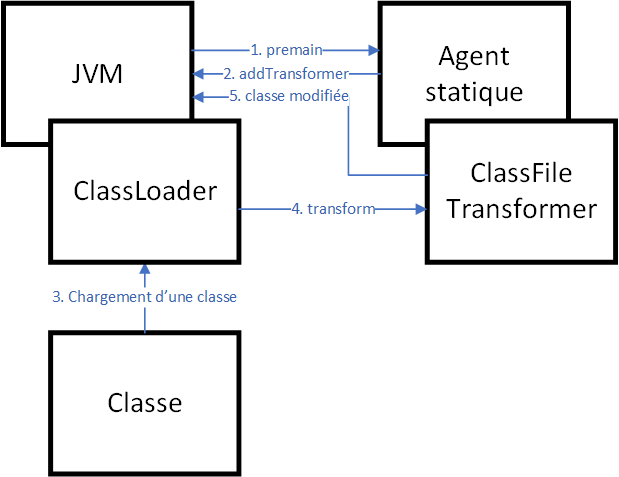
\includegraphics[width=.7\linewidth]{cojac/static_agent.png}
}
\captionof{figure}{Fonctionnement d'un agent statique}
\label{fig:cojac_static_agent}
\end{minipage}

\subsection{Agent dynamique}

Un agent dynamique est un \gls{Java-agent} qui est ajouté après le démarrage de l'application cible. Ceci rend la modification du programme plus complexe et nécessite une autre application pour insérer l'agent. L'ajout de l'agent se déroule en plusieurs étapes comme montré sur la Figure \ref{fig:cojac_dynamic_agent}:

\begin{enumerate}
    \item Une application pour ajouter l'agent doit être créée. Cette application doit s'attacher à la \gls{JVM} du processus dans lequel l'agent doit être inséré. Cette opération ne peut se faire que si l'application cible et l'application source sont sur des processus possédés par le même utilisateur pour des raisons de sécurité.
    \item L'application source charge ensuite l'\gls{Java-agent} dans l'application cible.
    \item Contrairement à l'agent statique, la \gls{JVM} appelle une autre méthode nommée \textit{agentmain}.
    \item L'agent enregistre ensuite son \textit{ClassFileTransformer}.
    \item Cette étape est facultative. Cependant, comme l'application cible a démarrée avant l'agent, elle a déjà chargée certaines classes. La méthode \textit{Instrumentation.\hspace{0pt}retransformClasses} permet de transformer les classes déjà chargées. Cependant, il y a quelques restrictions qui sont listées dans la documentation officielle de cette méthode \cite{java-instrumentation-retransform-documentation}. Pour chaque classe à retransformer, les étapes 6 à 9 seront à nouveau exécutées.
    \item Ensuite à chaque fois que la \gls{JVM} veut charger une nouvelle classe, le \textit{ClassLoader} lira le fichier \textit{.class} correspondant.
    \item Le \textit{ClassLoader} enverra ensuite le tableau de bytes qu'il vient de lire au \textit{ClassFileTransformer} qui pourra y apporter les modifications désirées.
    \item Une fois que le \textit{ClassFileTransformer} a modifié la classe, il la retournera la classe à la \gls{JVM}.
\end{enumerate}

\begin{minipage}{\linewidth}
\makebox[\linewidth]{
    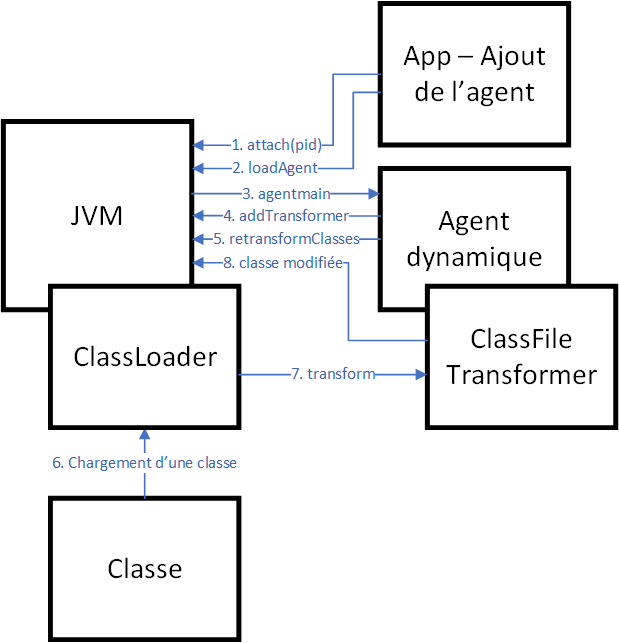
\includegraphics[width=.7\linewidth]{cojac/dynamic_agent.png}
}
\captionof{figure}{Fonctionnement d'un agent dynamique}
\label{fig:cojac_dynamic_agent}
\end{minipage}

\subsection{Synthèse}

Un \gls{Java-agent} permet de modifier le comportement de l'application cible sans en modifier le code source. Cette fonctionnalité permet de faire du profilage, de surveiller des applications ou de modifier le comportement d'une libraire propriétaire.

Les agents statiques et dynamiques ont des objectifs différents. Voici leurs avantages et inconvénients respectifs.

Les agents statiques possèdent les caractéristiques suivantes :

\begin{itemize}
    \item Le changement de l'agent statique nécessite de redémarrer l'application cible.
\end{itemize}

Les agents dynamiques possèdent les caractéristiques suivantes :

\begin{itemize}
    \item La retransformation de classes a d'importantes limitations. Celles-ci sont définies dans la documentation officielle de la méthode correspondante \cite{java-instrumentation-retransform-documentation}.
    \item L'agent peut être ajouté après que l'application ait démarré. Cette fonctionnalité permet, par exemple, de pouvoir obtenir des informations sur une application ayant un bug rare, inconnu ou qui se produit après un certain temps d'activité.
\end{itemize}


\section{Bytecode Java}
\label{sec:bytecode}

Tel que brièvement mentionné dans la section \ref{sec:agent_java} précédente sur les \glspl{Java-agent}, la \textbf{machine virtuelle Java} (\textbf{Java Virtual Machine} ou \textbf{\gls{JVM}}) utilise un seul langage: le \gls{Bytecode} Java. Bien qu'il soit possible de programmer en Java, en Kotlin ou encore en C pour nommer quelques exemples, la \gls{JVM} n'utilise que du \gls{Bytecode}.

Le nom de \gls{Bytecode} provient du fait que chaque code d'opération fait exactement 1 byte. Ceci limite fortement le nombre de codes d'opération disponibles à 256. Certains codes d'opérations peuvent être suivis de paramètres précisant l'opération à effectuer. Voici deux exemples de \gls{Bytecode} dont leur fonctionnement sera illustré plus loin. La première opération prend un byte en paramètre alors que la deuxième opération n'en prend pas.
\begin{minted}{text}
bipush 5
iadd
\end{minted}

Contrairement aux processeurs habituels, la \gls{JVM} utilise une pile au lieu de registres. Certaines opérations permettent de charger des informations sur la pile ou d'y retirer un élément pour le stocker dans une variable. Toutes les autres opérations prennent comme entrée les valeurs sur la pile et ajoutent le résultat sur cette même pile.

Voici un exemple de \gls{Bytecode} qui permet de mettre deux integers sur la pile et de les additionner:
\begin{minted}{text}
bipush 5
bipush 7
iadd
\end{minted}

\begin{minipage2}
L'exécution de ce \gls{Bytecode} est illustrée sur la Figure \ref{fig:cojac_bytecode_stack_addition}. Pour cet exemple, la pile est vide avant d'exécuter ces commandes. L'exécution se déroule en plusieurs étapes:

\begin{enumerate}
    \item Le nombre 5 est ajouté sur la pile.
    \item Le nombre 7 est ajouté sur la pile.
    \item L'addition consomme les deux nombres et ajoute le résultat sur la pile.
\end{enumerate}
\end{minipage2}

\begin{minipage}{\linewidth}% to keep image and caption on one page
\makebox[\linewidth]{%        to center the image
    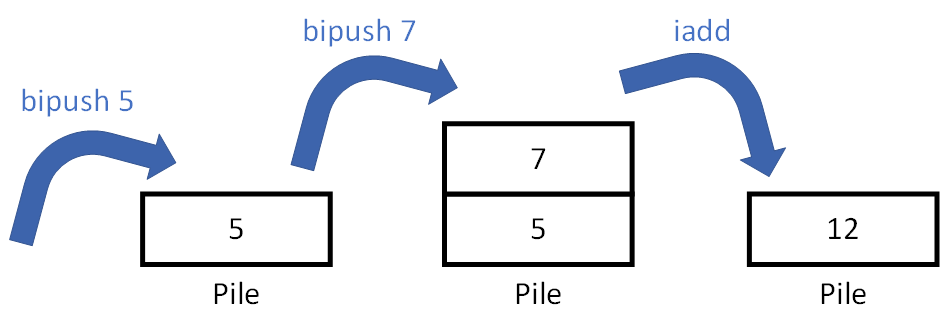
\includegraphics[width=.7\linewidth]{cojac/stack_addition_example.png}
}
\captionof{figure}{Addition de deux nombres en Bytecode Java}
\label{fig:cojac_bytecode_stack_addition}
\end{minipage}

Des informations plus complètes sont disponibles dans une conférence intitulée "Java Bytecode Crash Course" de David Buck, un ingénieur chez Oracle \cite{java-bytecode-video}.

Les spécifications de chaque instruction sont aussi définies dans la documentation officielle d'Oracle \cite{java-bytecode-documentation}.

\section{Intégration}
\label{sec:cojac_integration}

\gls{COJAC} propose deux manières d'intégrer une nouvelle fonctionnalité:

\begin{itemize}
    \item \textbf{\Gls{Behaviour}}: les opérations sur les floats et les doubles sont simplement remplacées par un appel de méthode. Ainsi, il est possible de changer le comportement de ceux-ci. Dans ce projet, il serait possible de mettre la partie réelle et la partie imaginaire dans un double et de modifier les opérations qui les utilisent.
    \item \textbf{Wrapper}: les floats et les doubles peuvent être remplacés par un objet (wrapper). Ce qui permet d'ajouter plus d'éléments dans le wrapper.
\end{itemize}

Le \gls{Behaviour} a les caractéristiques suivantes:

\begin{itemize}
    \item Le stockage est limité en taille (8 octets pour un double).
    \item Moins de modifications sont nécessaires. Toutes les opérations sur les doubles et les appels de la méthodes de la librairie standard doivent être modifiés. Il est également possible de convertir les floats en doubles. A ce moment, il y a beaucoup plus de modifications.
\end{itemize}

Le \gls{Wrapper} a les caractéristiques suivantes:

\begin{itemize}
    \item Le stockage est illimité.
    \item Beaucoup de modifications doivent être effectuées. Toutes les constantes, signatures de méthode, opérations, etc. doivent être adaptées parce qu'un type de base et un objet sont radicalement différents.
\end{itemize}

\subsection{Ajout d'un wrapper}

Pour ajouter un nouveau \gls{Wrapper} dans \gls{COJAC}, il faut créer une nouvelle classe dans le package \textit{com.github.cojac.models.wrappers}. Cette nouvelle classe doit hériter de la classe abstraite \textit{ACojacWrapper}. Il faut ensuite implémenter toutes les méthodes.

On peut ensuite tester le nouveau \gls{Wrapper} en suivant ces deux étapes:

\begin{enumerate}
    \item Créer le \gls{JAR} de \gls{COJAC}
    \item Démarrer l'application cible en donnant le \gls{JAR} créé précédemment comme \gls{Java-agent} et lui donner le \gls{Wrapper} à utiliser avec l'option \textit{-W}. Pour démarrer une application avec un \gls{Wrapper} nommé \textit{WrapperComplexNumber}, la commande suivante sera utilisée:
    \begin{minted}[breaklines]{shell}
java -javaagent:cojac.jar="-W cojac.WrapperComplexNumber" demo.HelloComplexNumber
    \end{minted}
\end{enumerate}

\subsection{Limitations}

La documentation de COJAC \cite{cojac-wiki-limitations} prévient que les \glspl{Wrapper} de \gls{COJAC} sont encore expérimentaux et qu'ils possèdent les limitations suivantes:

\begin{itemize}
    \item Il y a des problèmes dans les transitions entre le code utilisateur et la librairie standard Java. Par exemple, lors de l'utilisation de tableaux de nombres.
    \item Les "callbacks" de la bibliothèque Java vers le code utilisateur lorsque des nombres à virgule flottante sont transmis ne sont pas supportés.
    \item L'instruction \gls{Bytecode} \textit{invokedynamic} devrait fonctionner pour Java 8, mais cela n'est pas garanti. De plus, les nouvelles utilisations de cette instruction tel que mentionné dans la section \ref{sec:problem_cojac_instrumentation} ne sont pas supportés.
    \item L'utilisation de la \textit{Java reflection} n'est pas supportée.
    \item La conversion des types primitifs (float/double) et de leur \gls{Wrapper} original (Float/\hspace{0pt}Double) provoquent certains problèmes tels que des conflits de signatures de méthodes ou des erreurs de comparaison.
    \item L'implémentation des modèles n'est pas optimale. Par exemple, les appels à la librairie standard \textit{Math.*} ne calculent pas les valeurs aussi précisément que demandées.
    \item Il y a également un ralentissement important.
\end{itemize}

\subsection{Méthodes magiques}

\Gls{COJAC} offre aussi un mécanisme de méthodes magiques. Ces méthodes permettent à l'application cible d'utiliser du code de \gls{COJAC}. Le principe qui se cache derrière se mécanisme est bien documenté dans la section 5.4 d'un rapport précédent sur les nombres enrichis dans COJAC \cite{enriched-numbers}.

\section{Maven}

\gls{COJAC} utilise \gls{Maven} \cite{maven} pour créer le \gls{JAR}. \gls{Maven} est un outil d'automatisation pour gérer les dépendances et produire une application. Cet outil peut télécharger les dépendances, compiler le projet, exécuter les tests unitaires et d'intégration et déployer le projet. \gls{Maven} et Gradle sont les deux outils les plus souvent utilisés pour gérer les projets Java. Toute la configuration se trouve dans le fichier \textit{pom.xml}.

\subtitle{Debug}
\label{sec:cojac_maven_debug}

Lorsqu'il y a un problème avec \gls{Maven}, il y a plusieurs paramètres qui permettent d'obtenir plus d'informations. Cette section montre comment configurer ces paramètres sous IntelliJ et donne l'argument équivalent pour appeler \gls{Maven} en ligne de commande.

\begin{minipage2}
\subtitle{Ouvrir la fenêtre Maven}

Toutes les configurations effectuées ci-dessous seront effectuées depuis la fenêtre \gls{Maven} dans IntelliJ. Le bouton pour l'ouvrir se situe sous \textbf{View} $\rightarrow$ \textbf{Tool Windows} $\rightarrow$ \textbf{Maven} comme montré sur la Figure \ref{fig:maven_open_window}.
\end{minipage2}

\begin{minipage}{\linewidth}% to keep image and caption on one page
\makebox[\linewidth]{%        to center the image
    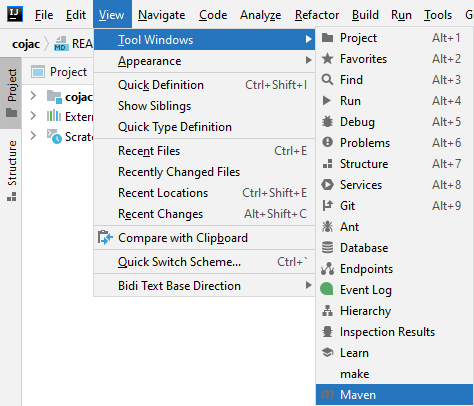
\includegraphics[width=.7\linewidth]{maven/open_maven_window.png}
}
\captionof{figure}{Bouton d'ouverture de la fenêtre \gls{Maven}}
\label{fig:maven_open_window}
\end{minipage}

\subtitle{Fenêtre Maven}

La fenêtre \gls{Maven} montre le contenu du projet avec les étapes du cycle de vie de la production de l'application comme le montre la Figure \ref{fig:maven_window}. Le bouton encadré sur l'image permet d'ouvrir les paramètres de \gls{Maven} qui seront utilisés plus tard. On peut également voir les plugins et les dépendances. Cette fenêtre permet aussi d'exécuter les étapes pour produire l'application. L'étape \textit{package} est suffisante pour générer le \gls{JAR}.

\begin{minipage}{\linewidth}
\makebox[\linewidth]{
    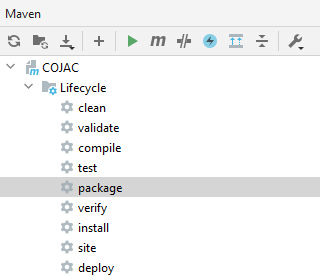
\includegraphics[width=.5\linewidth]{maven/maven_window_annotated.png}
}
\captionof{figure}{Fenêtre \gls{Maven}}
\label{fig:maven_window}
\end{minipage}

Une option peut être ajoutée pour afficher les messages de debug. Cette option est plus souvent utilisée lors du développement de \gls{Maven} ou d'un plugin \gls{Maven}. Cependant, elle peut également être utile pour trouver la source d'un problème difficile. Cette option est visible sur la Figure \ref{fig:maven_debug}. L'option en ligne de commande équivalente se nomme \textit{-{}-debug}.

\begin{minipage}{\linewidth}
\makebox[\linewidth]{
    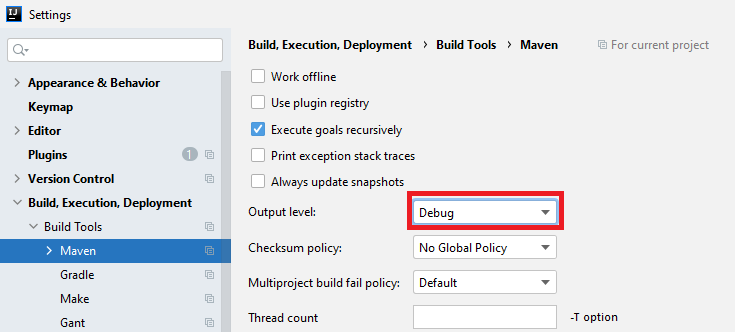
\includegraphics[width=\linewidth]{maven/maven_debug.png}
}
\captionof{figure}{Configuration d'affichage des messages de debug}
\label{fig:maven_debug}
\end{minipage}